\chapter{Не решённые и только-что решённые}


\setlength{\epigraphwidth}{.80\textwidth}
\epigraph{Мы должны знать --- мы узнаем!
}{--- Давид Гильберт (1862---1943)}

Плохая новость: эта глава может вас сломать.
Но есть и хорошая новость: нерешённая задача совсем не значит, что она неразрешима.
На самом деле две из нерешённых головоломок моей предыдущей книги были недавно решены.
Первая была особенно известной, и с ней произошло нечто поистине удивительное.

\subsection*{Ангел и дьявол Конвея}\rindex{Ангел и дьявол Конвея}

Ангел летает над бесконечной шахматной доской и время от времени
должен садиться на клетку.
Он может пролететь не более 1000 ходов
короля до очередного приземления.

Пока ангел в небе, дьявол, живущий под доской, может уничтожить любую клетку на свой выбор.

Сможет ли дьявол добиться того, чтоб ангелу было некуда приземлиться?

\medskip

Поразительно и непостижимо, но эта открытая тридцать лет головоломка, была внезапно решена
независимо и почти одновременно
\emph{четырьмя} людьми из четырёх разных стран \cite{10, 20, 40, 43}.

При этом идеи были по большей части схожими, и они не опирались на недавно разработанные новые методы.
Более того, все доказательства строились на наблюдениях, сделанных самим Джоном Конвеем ещё в 70-х.
Четверо решивших были:
Андраш Мате из Университета имени Этвёша Лоранда в Будапеште,
Брайан Боудич из Университета Саутгемптона,
Оддвар Клостер из SINTEF ICT в Осло
и Питер Гакс из Бостонского университета.
Было давно известно, что ангела мощности $p=1$ (который перемещается на один ход короля) можно победить.
Мате и Клостер показали, что ангел мощности $p=2$ выигрывает;
Боудич доказал, что достаточно мощности $p=4$,
а Гакс --- что \emph{какой-то} мощности $p$ достаточно.

Доказательства оказались достаточно простыми, так что Бела Боллобаш из Кембриджского университета и Университета Мемфиса, смог разобрать их на восхитительном одночасовом докладе в Университете Иллинойса.
Далее следует выжимка из его доклада и статьи Мате, доказывающей, что ангел мощности 5 выигрывает.

Идея показать, что если ангел выигрывает (в несколько более сильном смысле) против несколько более слабого противника, называемого \emph{добрым дьяволом}, то он сможет выиграть и против изначального (\emph{злого}) дьявола.
Как мы увидим, против доброго дьявола сработает удивительно простая стратегия.

Доброму дьяволу запрещено уничтожать клетку, на которую ангел мог бы прыгнуть ранее;
другими словами, все клетки на расстоянии не больше $p$ от любой ранее посещённой клетки нельзя уничтожить.

Ангел может выиграть в изначальной игре, если для любого $n$, он может уйти на расстояние $n$ ---
это легко проверить.
Мы хотим продемонстрировать, что если такое можно проделать с добрым дьяволом, то можно и со злым.

Предположим, у злого дьявола \emph{есть} стратегия, удерживающая ангела на расстоянии $n$ от начальной клетки.
Сейчас мы покажем, как добрый дьявол может сделать то же самое.
По данной последовательности ходов ангела, построим \emph{сокращённую} последовательность следующим образом.
Пусть $A_1$ --- самая ранняя клетка посещённая ангелом, с которой он мог бы прыгнуть на последнюю клетку $A_0$.
Удалим все ходы между $A_1$ и $A_0$.
Далее пусть $A_2$ --- самая ранняя клетка посещённая ангелом, с которой он мог бы прыгнуть прямо на~$A_1$.
Удалим все ходы между $A_2$ и $A_1$.
Продолжая таким образом, мы получаем сокращение исходной последовательности $A_k$, $A_{k-1}, \dots, A_1$, $A_0$, в котором ангел никогда не прыгает в точку, с которой мог бы попасть ранее.

Теперь заставим доброго дьявола реагировать на данную последовательность ходов так, как это сделал бы злой дьявол в ответ на сокращённую последовательность, с одним изменением --- если требуется съесть недозволенную клетку (или нужная клетка уже съедена), то вместо этого добрый дьявол съедает любую дозволенную.
Легко показать, что если данная последовательность работает против доброго дьявола (то есть, ангелу не приходится сесть на съеденную клетку), то сокращение этой последовательности срабатывает против злого.
То есть, если ангел сможет уйти на расстояние $n$, играя против доброго дьявола, то он сможет сделать то же самое и против злого, а значит, сможет выиграть.

\begin{figure}[htb!]
\centering
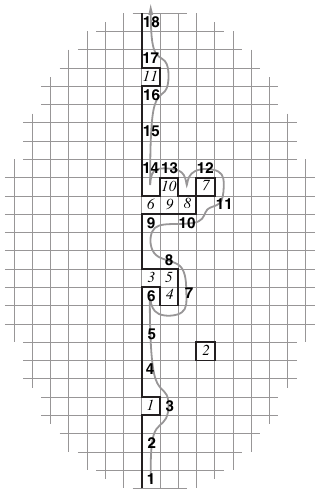
\includegraphics[scale=1]{pics/angel}
\caption{Стена отмечена чёрным, ангел --- жирным шрифтом, добрый дьявол --- курсивом.}
\label{pic:angel}
\end{figure}

Мы свели задачу к убеганию от доброго дьявола, а сделать последнее очень просто ---
ангел может даже позволить себе бегать, не прыгая, по несъеденным клеткам.
Он начинает на клетке, нижний левый угол которой находится в начале координат, и представляет себе стену вдоль линии $y = 0$.
Каждый раз, когда добрый дьявол съедает клетку, он возводит стену вокруг этой клетки.
Тем временем, на каждом ходу, ангел старается бежать на север вдоль стены, держа её слева от себя, пока это возможно.
Иногда ангелу придётся бежать на юг, чтобы обойти какой-то участок стены, но мощности $5$ 
хватает для того, чтобы продвигаться на север по крайней мере на единицу за каждый сделанный шаг.
Отсюда следует, что ангел мощности $5$ может уйти произвольно далеко.
Проделав дополнительную работу, можно убедиться, что и мощности $2$ достаточно.
На рис. \ref{pic:angel} показан возможный путь ангела мощности~$2$.

Стратегия ангела, описанная выше, конечно же \emph{не работает} против злого дьявола, который может, например, подготовить ловушку для ангела далеко по оси $y$ --- дьявол заманит ангела в конец полуострова, окружённого морем съеденных клеток, а затем отрежет его от берега.
Хороший дьявол не может этого сделать, ведь ему нельзя уничтожить вход на полуостров после того, как ангел туда прошёл.

К сожалению, то как стратегию убегания от доброго дьявола можно превратить в стратегию против злого, объяснить довольно трудно, даже при том, что построение выше довольно прямолинейно.
От части это и объясняет, почему головоломка не решалась так долго и подтверждает при этом, что сокращения --- мощный инструмент.

\begin{addedbytheeditors}
\textbf{Редакторам:} Мутный оригинал и мутный перевод. Сам в доказательтве не разбирался, но может кому-то это интересно и этот кто-то всё перепишет?
\end{addedbytheeditors}


\medskip

Следующей головоломке ещё далеко до полного решения,
однако до недавнего времени про неё вовсе ничего не было доказано.

\subsection*{Затор}\rindex{Затор}

Вершины бесконечной решётки на плоскости выбираются независимо с
фиксированной вероятностью $p\in (0,1)$.
В каждую из выбранных вершин
помещают автомобиль, направленный либо на север, либо на восток;
в каждом случае направление выбирается независимо подбрасыванием монеты.

Движение регулируется светофорами, которые включают поочерёдно:
«зелёный-восточный» и «зелёный-северный».
При включённом
зелёном-восточном каждый автомобиль, направленный на восток, правая
соседняя вершина от которого не занята, перемещается в эту вершину;
остальные (в том числе заблокированные другим восточным автомобилем),
остаются на месте.

Когда включается зелёный-северный, каждый незаблокированный
автомобиль, направленный на север, перемещается на одну вершину в
северном направлении.

Эксперименты показывают, что если $p$ меньше определённого
критического значения $p_0$, то автомобили постепенно разъедутся
(при этом каждый автомобиль будет иметь предельную скорость,
равную скорости автомобиля, который вовсе не блокируется).
Но когда
$p> p_0$, происходит обратное: автомобили попадают в безнадёжный
затор, то есть каждый автомобиль совершает лишь конечное число переездов
и останавливается навсегда.

Эту модель движения транспорта на перекрёстке двух крупных односторонних улиц представили О. Бихам, А. А. Миддлтон и Д. Левин в 1992 году \cite{6}.
Её странное поведение привлекло много внимания.
%библиографию можно найти по ссылке http://cui.unige.ch/spc/Bibliography/traffic.html.
%недоступная и незархивированя ссылка??? 

\begin{figure}[htb!]
\centering
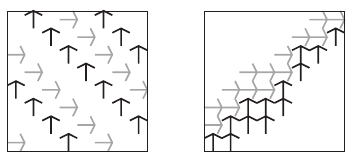
\includegraphics[scale=1]{pics/gridlock}
\caption{Свободное движение слева и затор справа.}
\label{pic:gridlock}
\end{figure}

На рис. \ref{pic:gridlock} изображены конечные части свободной конфигурации и конфигурации с затором, каждая из которых типична для того, что появлялось в экспериментах, проводимых Раисой Де Соуза \cite{15}, ныне преподаёт в Университете Калифорнии в Дэвисе.

Весной 2005 года в Исследовательском институте математических наук в Бёркли Омер Ангел, Эндер Холройд и Джеймс Мартин сделали первый существенный шаг: они доказали существование фазы затора.
Другими словами, при достаточно высокой плотности машин произойдёт затор --- каждая машина совершит лишь конечное число переездов.
Мы не приводим доказательство, но оно весьма изобретательно использует теорию перколяций, и с ним очень стоит ознакомиться \cite{2}.

\medskip

Конечно же, каждый раз, когда решается одна математическая задача, появляются три новые.
Думаю, что следующие несколько красавиц заслуживают внимания.

\subsection*{Упаковка прямоугольников}\rindex{Упаковка прямоугольников}

Дан конечный набор точек в квадрате, включающий его нижний левый угол.
Разрешается выбрать набор непересекающихся прямоугольников, лежащих в квадрате, левые нижние вершины которых образуют данный набор точек.
Можно ли выбрать прямоугольники так, чтобы их общая площадь была не меньше половины площади всего квадрата?

\medskip

Эту сбивающую с толку задачу я узнал больше десяти лет назад,
о ней мне сообщил Билл Паллиблэнк (математик и администратор) из IBM, который не помнил, откуда она к нему попала.
С тех пор задача всплывала то там, то сям, но мне не удалось найти более ранний источник.
В июне 2004 года она появилась на веб-странице головоломок IBM \cite{ponder-this}, но так и осталась нерешённой.
Я даже не могу доказать то, что прямоугольники могут покрыть 1\% площади квадрата.

\begin{figure}[htb!]
\centering
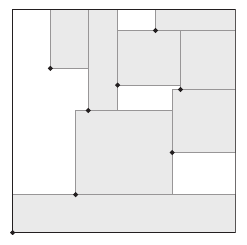
\includegraphics[scale=1]{pics/square}
\caption{Прямоугольники покрывают больше половины площади.}
\label{pic:square}
\end{figure}

На рис. \ref{pic:square} изображена конфигурация точек вместе с подходящим набором прямоугольников.

\subsection*{Произведения и суммы}\rindex{Произведения и суммы}

Можно ли раскрасить неотрицательные целые числа $\{0,1,2,\dots\}$ конечным числом цветов так, чтобы сумма $x+y$ и произведение $xy$ любых двух целых чисел были разных цветов?

\medskip

Эта задача была предложена Дэвидом Гэлвином, постдоком в Университете Пенсильвании.
Вроде как известен набор из шести чисел, таких, что любые два из них являются произведением и суммой некоторой пары, так что для раскраски потребуется по крайней мере шесть цветов.
С другой стороны, известно, что не существует произвольно больших наборов чисел с указанным свойством.

\medskip

Следующая загадка связана с игрой под названием «Социальное давление», придуманной Борисом Алексеевым из Университета Джорджии.
В неё активно играла команда США недавней математической олимпиады.

\subsection*{Социальное давление}\rindex{Социальное давление}

Двум игрокам сдают по некоторому числу карт, сначала \emph{в открытую} (рубашкой вниз).
На каждой карте написано целое число, все числа различны.
В каждом раунде игроки одновременно выкладывают по карте;
старшая карта сбрасывается, а младшая передаётся другому игроку.
Проигрывает тот у кого кончились карты.

При увеличении числа сдаваемых карт,
какова предельная вероятность того, что у одного из игроков будет выигрышная стратегия?

\medskip

Борис (как и я) подозревает, что эта вероятность стремится к нулю, но анализ этой простой вариации игры в пьяницу кажется сложным.

\begin{addedbytheeditors}
\textbf{Редакторам:} Не смог понять с чего игра называется peer pressure.
\end{addedbytheeditors}

\medskip

А вот неожиданная загадка от Стива Хедетниеми из Университета Клемсона:

\subsection*{Покрытие ферзями}\rindex{Покрытие ферзями}

Пусть $f(n)$ --- минимальное число ферзей, которые можно расставить на доске размера $n \times n$ так, чтобы каждая клетка была под ферзём или под боем ферзя.
Верно ли, что $f(n + 1) \geqslant f(n)$ при всех~$n$?

\medskip

Есть уйма головоломок о расстановке шахматных фигур (обычно ферзей или коней) на доске $n \times n$.
Ферзей обычно стараются расставить как можно большее, чтоб ни один не бил другого.
Однако нам нужно наименьшее число ферзей, контролирующих всю доску.
Трудно поверить, что для контроля меньшего числа клеток может понадобиться больше ферзей, однако на большей доске есть больше мест, откуда ферзь может контролировать свои владения, и это нужно учитывать!

\medskip

А вот увлекательная, но на самом деле довольно серьёзная головоломка, которая уже многие годы сбивает с толку специалистов по оптимизации.

\subsection*{Встреча}\rindex{Встреча}

Двое приятелей потеряли друг друга в огромном торговом центре. %???The Mall of America (аббревиатура: MOA, с англ. — «Молл Америки») — торговый центр, расположенный в Миннесоте в пригороде Миннеаполиса, неподалеку от аэропорта Миннеаполис/Сент-Пол. Он был открыт в 1992 году и является одним из крупнейших торговых центров мира.
На поиск в одном магазине у них уходит по 15 минут,
при этом время перемещения от одного магазина к другому ничтожно мало
(торговый центр --- удобно устроенный огромный многоэтажный квадрат).
Они не договорились о месте встречи и не определили заранее, кто будет искать, а кто останется на месте.
Как им следует действовать, чтобы минимизировать ожидаемое время поиска?

\medskip

Если один из них ищет, а другой ждёт на месте, то в среднем потребуется проверить $n/2$ магазинов, где $n$ --- число магазинов в торговом центре (предполагается, что оно большое).
Однако наши правила запрещают протокол, нарушающий симметрию;
нельзя, например, чтоб младший искал, а старший сидел на месте.
Если оба ищут, то в среднем потребуется $n$ шагов, до того как они окажутся в одном и том же магазине в одно и то же время и найдут друг-друга.

В 1976 году этот вопрос был сформулирован (в других словах) Стивом Альперном из Лондонской школы экономики.
О нём и некоторых других вопросах можно почитать на веб-сайте Ричарда Вебера из Кембриджского университета \cite{weber}.
Вебер и Э. Дж. Андерсон предложили алгоритм, согласно которому каждый из приятелей бросает изогнутую монетку, решая с вероятностью около $0{,}2475$ оставаться на месте или же проверять магазины в случайном порядке,
и через каждые 15 минут, а в случае неудачи, повторять процесс.
Это приводит к успеху в среднем за $0{,}8289n$ шагов.
Однако никто не смог доказать то, что лучшего добиться нельзя.

\begin{addedbytheeditors}
\textbf{Редакторам:} Добавил «через каждые 15 минут,»
\end{addedbytheeditors}


\subsection*{Подкрученный прямоугольник}\rindex{Подкрученный прямоугольник}

Вы, наверное знаете, что ленту Мёбиуса можно получить из длинной прямоугольной бумажной ленты,
склеив её концы с подкруткой на пол оборота.
А какой длины нужна полоса?
Иными словами, 
какие пропорции прямоугольника оптимальны для склейки ленты Мёбиуса, без растяжения или сгибания?

Дмитрий Фукс и Сергей Табачников представили эту головоломку \cite[Лекция 14]{19} вместе с доказательством, что отношение длины к ширине не может быть меньше $\pi/2 \sim 1{,}57$, и примером для любого отношения больше $\sqrt{3} \sim 1{,}73$.
Однако точный ответ неизвестен.

\begin{addedbytheeditors}
Задача решена Ричардом Шварцем \cite{schwartz}; отношение обязано превосходить $\sqrt{3}$.
\end{addedbytheeditors}


\subsection*{Торговые автоматы}\rindex{Торговые автоматы}

Несколько торговых автоматов в местной игровой зоне работают случайным образом,
иногда выдавая много жевательных резинок за раз, а иногда не выдавая вообще ничего.
Однако в среднем каждый автомат выдаёт одну жевательную резинку за раз.
Какова максимально возможная вероятность того, что все $n$ автоматов за раз выдадут больше чем $n$ жевательных резинок?

\medskip

Эта головоломка (сформулированная в терминах независимых случайных переменных) принадлежит Ури Фейге из Microsoft Research.
Кажется оптимальным заставить каждый автомат выдавать $n + 1$ жевательную резинку с вероятностью $1/(n + 1)$,
а иначе ни одной.
В этом случае мы получим больше, чем $n$ жевательных резинок если хоть один автомат сработает.
Это происходит с вероятностью
\[1-(1-\tfrac1{n+1})^{n+1},\]
которая близка к $1 - 1/e \sim 63\%$, при больших $n$.
Пока никто не придумал ничего лучшего.
Сам Фейге доказал, что вероятность получить более чем $n$ жевательных резинок не может превысить $12/13$.

Разве может такая задача быть трудной?

\subsection*{Круги на плоскости}\rindex{Круги на плоскости}

Дано множество открытых единичных кругов, которое тысячекратно покрывает плоскость;
то есть, каждая точка $\mathbb{R}^2$ покрывается как минимум тысячью кругами.
Докажите, что круги можно раскрасить в красный и синий цвета так,
чтобы красные и синие круги по отдельности покрывали всю плоскость.

\medskip

Придумал эту замечательную задачу Янош Пах из Нью-Йоркского университета (он же и главный специалист по ней).
В своей статье \cite{46} он доказал, что для любого симметричного многоугольника $P$ и любого положительного целого числа $r$ существует число $k$, такое что любое $k$-кратное покрытие плоскости параллельными переносами $P$ можно разбить на $r$ покрытий.
Но если многоугольник заменить на круг, то даже при $r = 2$ неизвестно найдётся ли такое $k$.

Я считаю, что $k = 4$ должно хватить.
А вы, что скажете?
